\documentclass[11pt, oneside]{article}   	% use "amsart" instead of "article" for AMSLaTeX format

% \usepackage{draftwatermark}
% \SetWatermarkText{Draft}
% \SetWatermarkScale{6}
% \SetWatermarkLightness {0.90} 
%\SetWatermarkColor[rgb]{0.7,0,0}


\usepackage{geometry}                		% See geometry.pdf to learn the layout options. There are lots.
\geometry{letterpaper}                   		% ... or a4paper or a5paper or ... 
%\geometry{landscape}                		% Activate for for rotated page geometry
%\usepackage[parfill]{parskip}    		% Activate to begin paragraphs with an empty line rather than an indent
\usepackage{graphicx}				% Use pdf, png, jpg, or eps� with pdflatex; use eps in DVI mode
								% TeX will automatically convert eps --> pdf in pdflatex		
\usepackage{amssymb}
\usepackage{mathrsfs}
\usepackage{hyperref}
\usepackage{url}
\usepackage{subcaption}
\usepackage{authblk}
\usepackage{amsmath}
\usepackage{mathtools}
\usepackage{graphicx}
\usepackage[export]{adjustbox}
\usepackage{fixltx2e}
\usepackage{hyperref}
\usepackage{alltt}
\usepackage{color}
\usepackage[utf8]{inputenc}
\usepackage[english]{babel}
\usepackage{float}

 
\newtheorem{theorem}{Theorem}[section]
\newtheorem{corollary}{Corollary}[theorem]
\newtheorem{lemma}[theorem]{Lemma}

\newcommand{\argmax}{\operatornamewithlimits{argmax}}
\newcommand{\argmin}{\operatornamewithlimits{argmin}}


\title{Comments on "Tableless Routing"\footnote{This report is a deliverable for Project Number HE2017070001.}}
\author{David Meyer \\
dmm@1-4-5.net}

\date{Last update: \today}							% Activate to display a given date or no date


\begin{document}
\maketitle

\section{Introduction} 
\label{sec:intro}
The document provides a review of the "Tableless Routing" deck that was discussed on 09/19/2018. 

\bigskip
\noindent
The approach taken in this document will be to review each slide and provide comments where useful. 
These comments will be organized into three categories: 

\begin{itemize}
\item Feedback the technical aspects of each slide. I will include the slide where doing so would provide additional information
\item Feedback  on where we might find colleagues (industry, academia, or other)
\item Comparison to competitive approaches
\item Marketing strategies
\end{itemize}

\bigskip
\noindent
I will analyze the deck slide by slide, providing comments where appropriate. Here page number is equivalent 
to slide number. I will also include a section on Nits (editorial and non-technical comments) where appropriate.

\subsection{Introductory Comments on Graph Neural Networks for the Routing}
\label{subsec:gnn}
While I found the Graph Neural Networks and their use in routing  \cite{Scarselli:2009:GNN:1657477.1657482,DBLP:conf/sigcomm/GeyerC18}  interesting, I also  I found a few aspects of proposed 
protocol troublesome. First, nodes (routers) "cold-start" from some fixed-point state of the GNN. That seems relatively innocuous. However, nodes then update their routing state using the routing 
state of their neighbors. This seems very distance vector-like, and so I would expect similar problems (e.g., counting to infinity, split horizon, etc). 

\begin{figure}
\center{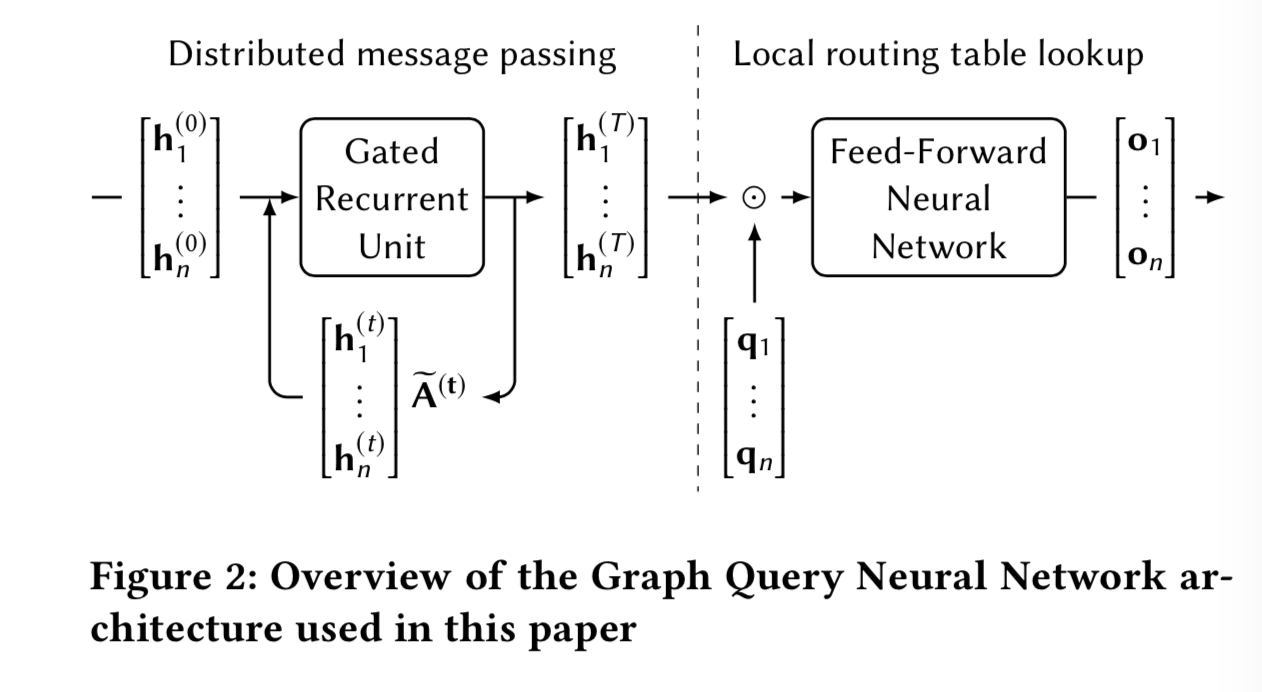
\includegraphics[scale=0.5, frame] {images/figure2.png}}
\caption{Figure 2 from \cite{DBLP:conf/sigcomm/GeyerC18}}
\label{fig:figure2}
 \end{figure}


\bigskip
\noindent
Second, the authors use dropout \cite{Srivastava:2014:DSW:2627435.2670313}  to regularize the training of the GNN. The idea here is that dropping out random links \footnote{The graph
is represented as an adjacency matrix.} during each training epoch (or whatever) effectively models packet loss, link failure, and router failure (or any other Byzantine failure, really). I'm skeptical 
that this approach can actually handle all of these failure modes.

\bigskip
\noindent
Third, the approach is to simulate a routing protocol on the graph (network) to generate the $\big [ \mathbf{h}^{(T)}_1,\hdots, \mathbf{h}^{(T)}_n \Big ]^\text{T} \odot \big [ \mathbf{q}_1,\hdots, \mathbf{q}_n \big ]^\text{T} \to \text{output port}$ mapping that is subsequently  used for supervised training of the Feed-Forward Neural Network (FFNN) in Figure \ref{fig:figure2}. 
So you need a routing protocol to find the output ports in the first place.

\bigskip
\noindent
The three aspects of the routing solution mentioned above make the entire approach less compelling. The question I would expect would relate to why this approach is better than just using OSPF 
\cite{rfc2328} (or whatever), since I already have to run such a protocol in simulation to build the dataset for supervised training.


\bigskip
\noindent
Finally, I would expect that "traditional" routing protocol engineers (IS-IS, BGP, etc) will argue against such an approach. The obvious arguments are that (i). the approach above is far more complex (and perhaps
less computationally efficient)  than existing shortest-path routing algorithms and (ii). given the probabilistic nature of machine learning algorithms, existing protocols can be shown to be deterministically correct,
while the machine learning approach can provide only probabilistic bounds.


\subsection{Comments on Routing Table Size as a Problem to Solve}
\label{subsec:table_size}

A few "historical" comments here. First, are \emph{routing table size} and \emph{IP lookup time} still compelling problems? Current day route processors (RPs) have plenty of DRAM, 
unlike the late 1990s/early 2000s, where routing table size and growth were critical concerns. So it is not clear that inter-domain routing table size is currently a problem. In addition, 
during our discussion of this deck (on 09/19/2018) it was stated that this scheme was designed for intra-domain routing, where table size really hasn't been a problem \footnote{On 
the other hand, IGP adjacency state has in the past been
as scaling problem.}.

\bigskip
\noindent
In addition, it is not clear how "table-oriented" functionality would be achieved. Such functionality includes various \emph{Virtual Private Network}, or VPN technologies \footnote{For example, how
would Virtual Routing and Forwarding (VRF) or multicast be supported?}.

\bigskip
\noindent
Another overview comment relates to \emph{IP lookup time}. It is not clear that this is a current problem either. The example I gave was MPLS (former Tag Switching). In this case one of the 
original objectives was to reduce IP lookup time from something like $O(n \log n)$ for trie-based lookup (depending on the exact shape of the trie)  to $O(1)$ for a 32-bit label lookup. It was 
learned, however, that since the IP lookup path was already so highly optimized that fixed length lookup really didn't speed up the overall lookup time.  

\bigskip
\noindent
Finally, I'm wondering if we can use the tableless approach in \emph{inter-domain} routing to infer bogus or hijacked prefixes. If we could do this accurately it might provide a 
lightweight alternative (or augmentation) for the RPKI \cite{rfc6810}. More work would be required here, and the IETF would be a reasonable place to do this work.

\bigskip
\noindent
This remainder document is organized as follows: Each of the following sections refers to a slide on which I have comments. Finally, Section \ref{sec:conclusions} provides a few conclusions.

\section{Slide 2}
\label{sec:slide2}


% \begin{figure}
% \center{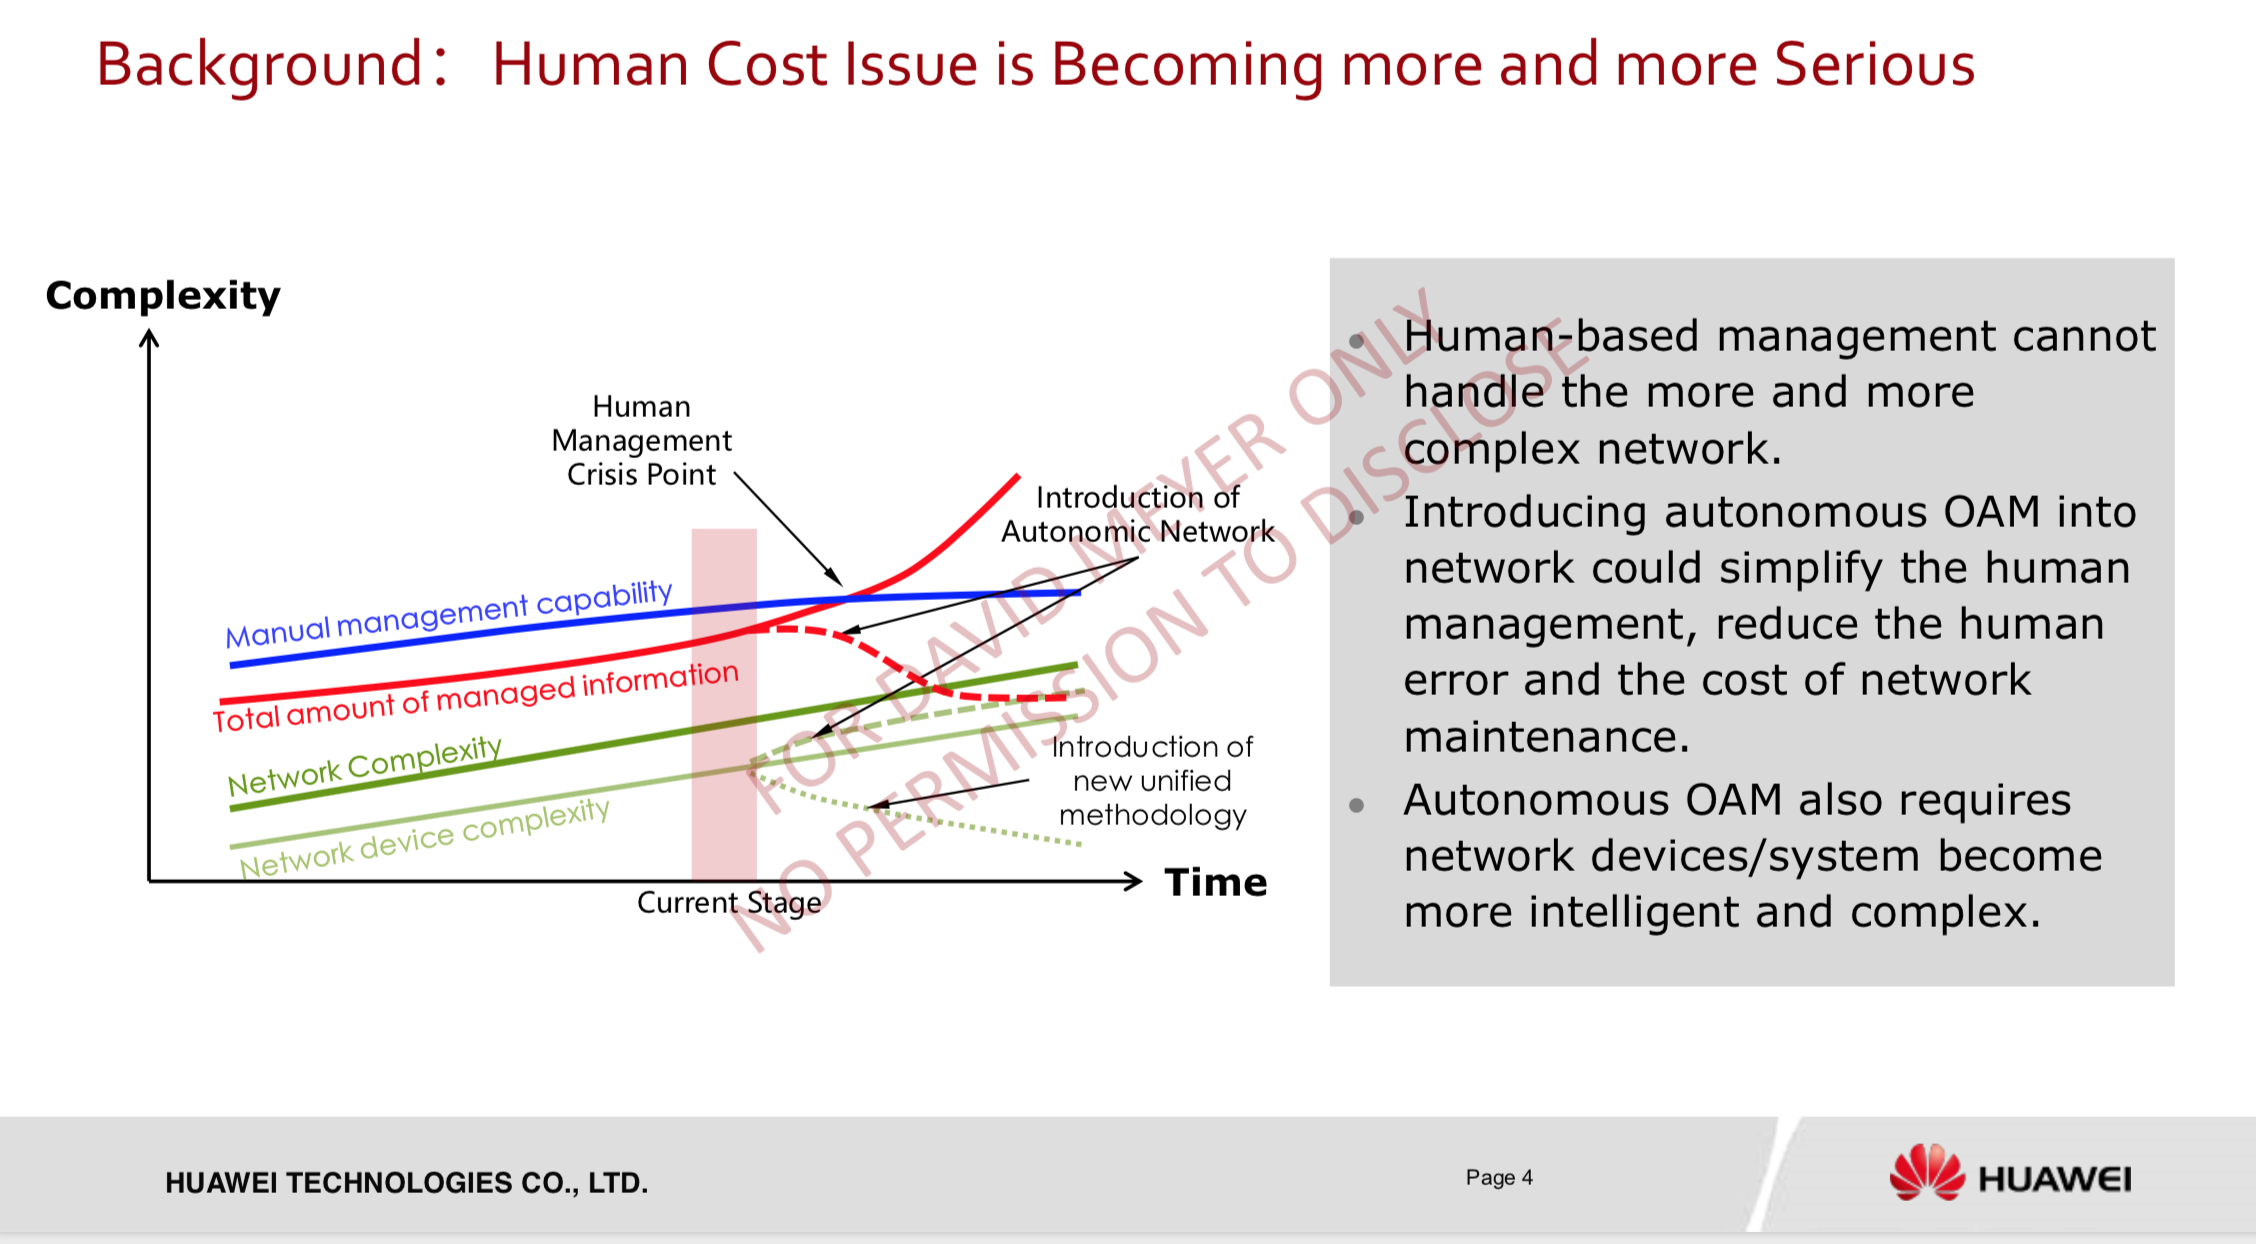
\includegraphics[scale=0.35, frame] {images/slide4.png}}
% \caption{Slide 4}
% \label{fig:slide4}
% \end{figure}


\subsection{Technical Feedback}
\label{slide2:technical_feedback}
Slide 2 outlines the motivation for tableless routing: 

\bigskip
\noindent

\begin{itemize}
\item Delay: Lower lookup latency
\item Chip Area Cost:  Lower (on-chip) memory requirements
\item Lookup bandwidth: This one isn't clear but it seems that if you don't have on-chip tables you don't need to access them.
\end{itemize}

\bigskip
\noindent
As mentioned above, it is not clear that lowering delay or table space is compelling. However, repurposing on-chip area that would have been used for on-chip
tables \emph{could be} motivating. More research on this point is required.

\bigskip
\noindent
More specifically, items 2 (Area cost) and 3 (Bandwidth) overlap significantly.  From my perspective Area cost is clear. The Bandwidth item (3) needs further
refinement.  It seems that the idea is that if you don't have tables that you need to lock or synchronize then various pipelines, both on-chip and
between chips, will be simpler. While slides 3-4  address this point to some extent, the difference is not crisp.  Hence we need to clarify the difference between items 2 and 3. 


\subsection{Possible Collaborators}
\label{slide2:possible_collaborators}
Large mobile operators would be have the best information here. This is largely due to their use of IPv6 and the continuing deaggregation 
makes them idea candidates for feedback on tableless routing.

\subsection{Marketing Strategies}
\label{slide2:marketing_strategies}
As mentioned above, more research in both the technology space and into the economics of the cost/benefit tradeoffs is required before any
marketing would be appropriate.

\subsection{Nits}
\label{slide2:nits}
N/A


\begin{figure}[t]
\center{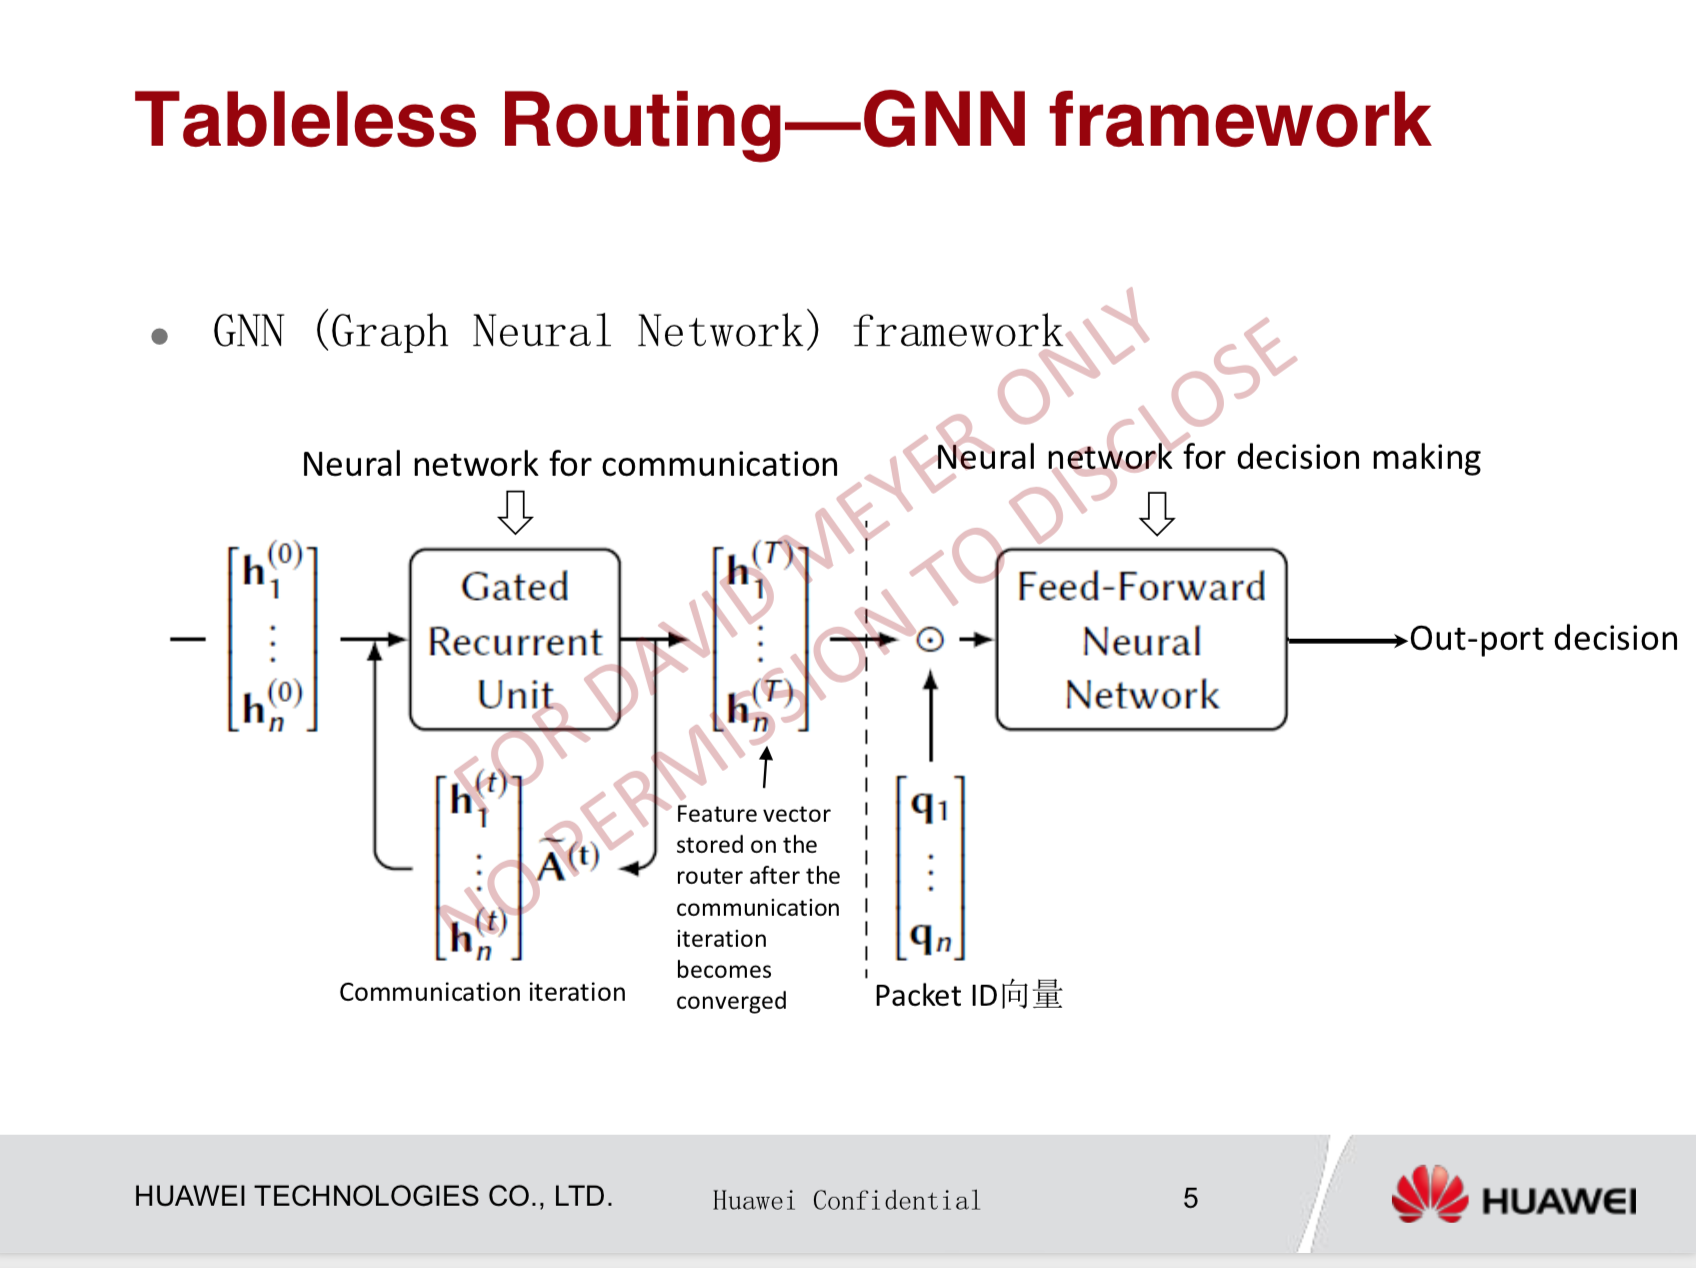
\includegraphics[scale=0.4, frame] {images/slide5.png}}
\caption{Slide 5}
\label{fig:slide5}
\end{figure}


\section{Slide 5}
\label{sec:slide5}
Slide 5 introduces the Graph Neural Network (GNN) architecture \cite{Scarselli:2009:GNN:1657477.1657482,DBLP:conf/sigcomm/GeyerC18} for tableless routing. 
The basic idea is to use the  Gated Recurrent Unit (GRU) \cite{2017arXiv170105923D} (a Recurrent Neural Network (RNN) variant) to learn a feature vector 
$\Big [ \mathbf{h}^{(T)}_1,\hdots, \mathbf{h}^{(T)}_n \Big ]^\text{T}$. This is the terminal internal state of the GRU
at convergence. That is, the network is trained with the iterative  Almeida-Pineda algorithm \cite{PhysRevLett.59.2229} which works by running the propagation 
of the hidden representation to convergence, and then computing gradients based upon the converged solution. This is depicted in 
Figures  \ref{fig:figure2} and \ref{fig:slide5}. Each iteration of the Almeida-Pineda algorithm is called a "communication iteration" on Slide 5.
Note that as mentioned above, a key idea here is that  training with \emph{dropout} \cite{Srivastava:2014:DSW:2627435.2670313} actually "ensambles" all of 
the possible networks and hence handles all possible link (and other) failures \footnote{See Slide 7; note that this is point is neither described nor proved.}. 



\bigskip
\noindent
This feature vector is then combined with a packet ID vector $\big [ \mathbf{q}_1,\hdots, \mathbf{q}_n \big ]^\text{T}$ by \emph{element-wise} multiplication (indicated by the
$\odot$ symbol) to form the input to a Feed Forward Neural Network (FFNN) which maps its input to output port. That is
\begin{equation*}
\big [ \mathbf{h}^{(T)}_1,\hdots, \mathbf{h}^{(T)}_n \Big ]^\text{T} \odot \big [ \mathbf{q}_1,\hdots, \mathbf{q}_n \big ]^\text{T} \to \text{output port}
\end{equation*}

\subsection{Technical Feedback}
\label{slide5:technical_feedback}
As mentioned above, there are a few technical issues here. See Section \ref{subsec:gnn} and \ref{subsec:table_size}. Compelling answers to the questions
there are needed.

\bigskip
\noindent
There is also an apparent bug in the feedback loop depicted in Figure 2 of \cite{DBLP:conf/sigcomm/GeyerC18}. In particular, assuming

\begin{equation*}
\begin{bmatrix}
           \textbf{h}_{1}^{(t)} \\
           \vdots \\
           \textbf{h}_{n}^{(t)}
         \end{bmatrix}
         \widetilde{\textbf{A}}^{(t)}
\end{equation*}

\bigskip
\noindent
is an inner-product \footnote{The inner-product of $\textbf{u}$ and $\textbf{v}$ is typically denoted with angle brackets: $\langle \textbf{u}, \textbf{v} \rangle$.}, then the 'shapes" are wrong. 
That is, $ \big [ \textbf{h}_{1}^{(t)}, \hdots,  \textbf{h}_{n}^{(t)} \big ]^{\text{T}}$ is of dimension $n \times 1$ while $\widetilde{\textbf{A}}^{(t)}$
is of dimension $n \times n$. For the output to be of dimension $n \times 1$ (input to the GRU), we would need 
\begin{equation*}
\widetilde{\textbf{A}}^{(t)}
\begin{bmatrix}
           \textbf{h}_{1}^{(t)} \\
           \vdots \\
           \textbf{h}_{n}^{(t)}
         \end{bmatrix}
\end{equation*}

\bigskip
\noindent
That is, $\big \langle n \times n, n \times 1 \big \rangle  \rightarrow n \times 1$. Slide 5 (Figure \ref{fig:slide5}) retains this apparent error.



\subsection{Possible Collaborators}
\label{slide5:possible_collaborators}
As I mentioned I find this approach very interesting and the possibility for other uses of this technology seem to be many. For example, I mentioned the possibility of 
a lightweight alternative to the RPKI  based on this technology might be possible. However, this idea would have to be fleshed out and tested.

\subsection{Marketing Strategies}
\label{slide5:marketing_strategies}
Because of my comments in Section \ref{slide5:possible_collaborators} it would seem premature to engage in marketing at this time.

\subsection{Nits}
\label{slide5:nits}
N/A



\begin{figure}[t]
\center{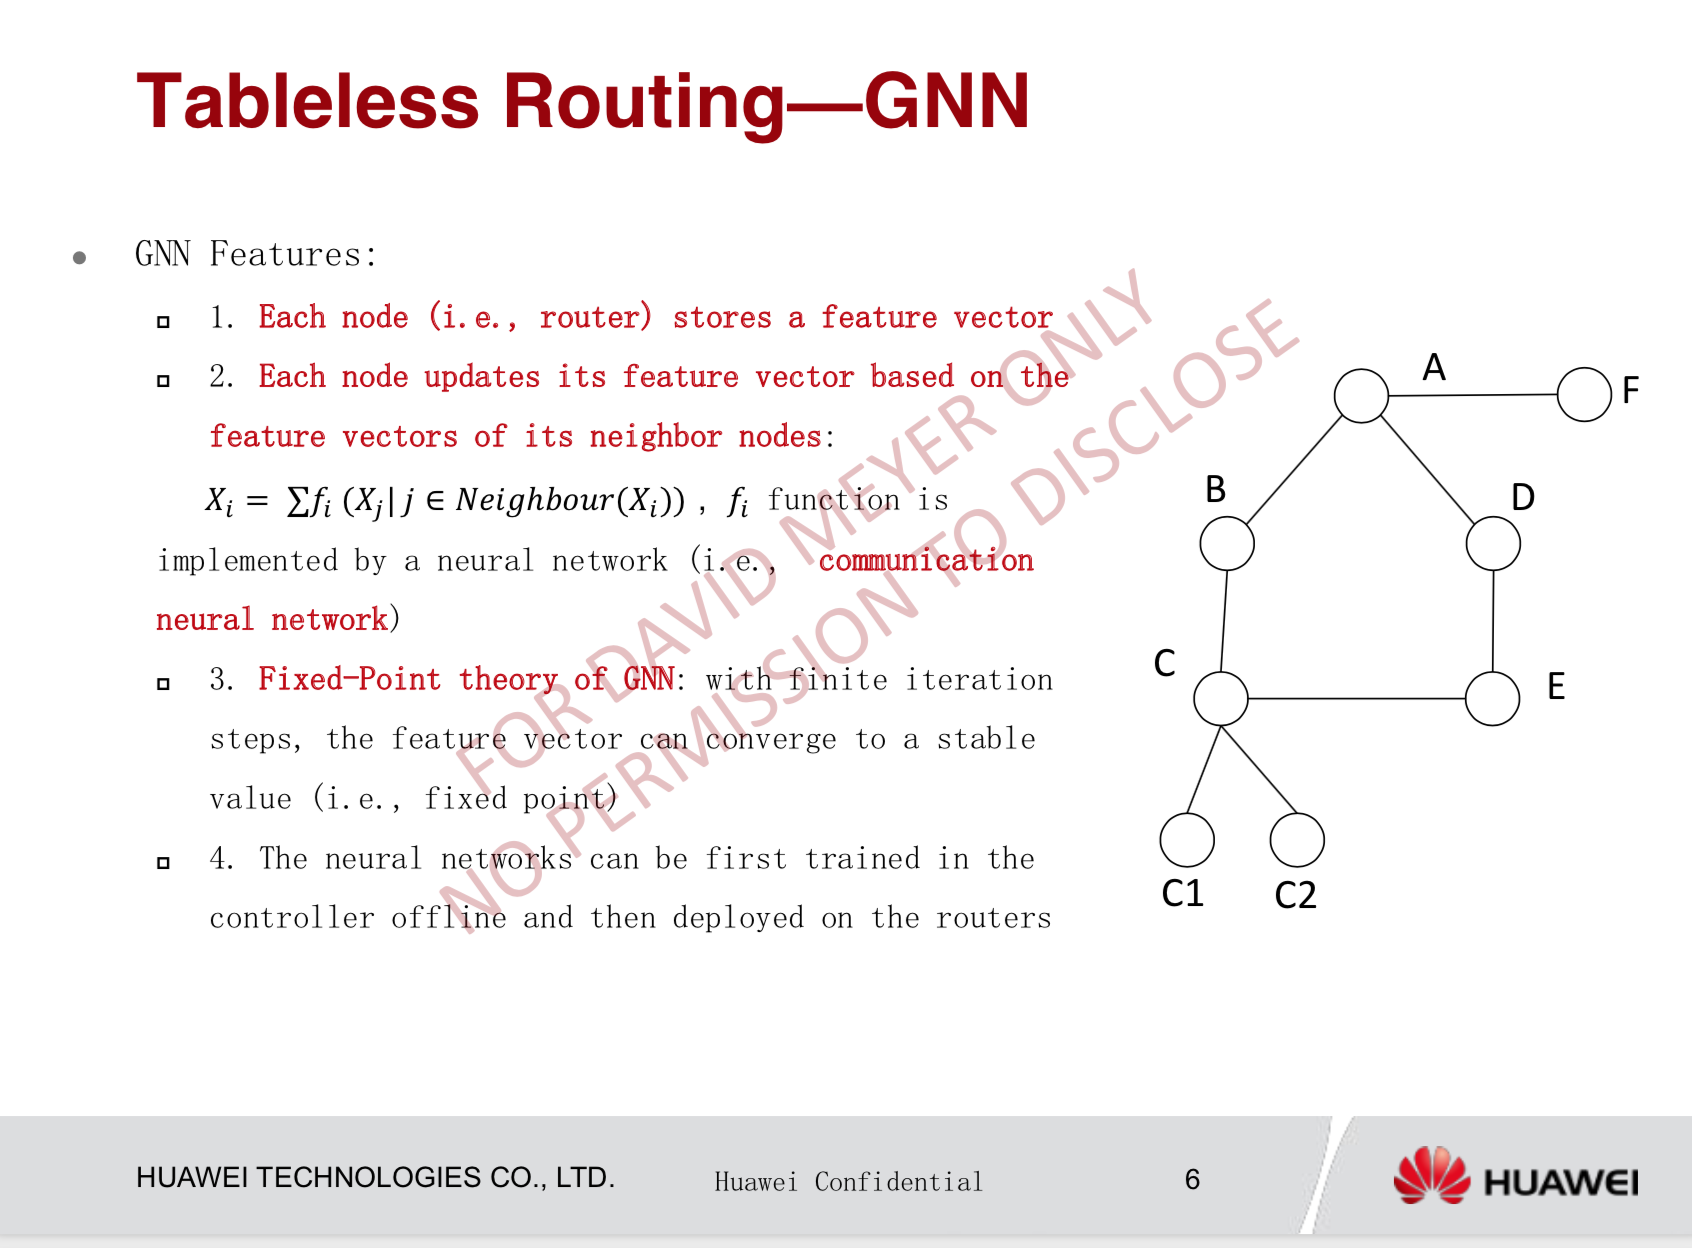
\includegraphics[scale=0.4, frame] {images/slide6.png}}
\caption{Slide 6}
\label{fig:slide6}
\end{figure}


\section{Slide 6}
\label{sec:slide6}
Slide 6 introduces an algorithm for dynamically updating a nodes feature vector as well as some important properties properties of the GNN.

\subsection{Technical Feedback}
\label{slide6:technical_feedback}
Sub-bullet 2 appears to be incorrect. Instead of 

\begin{equation*}
X_i = \sum f_i(X_j  | j \in \text{Neighbors}(X_i))
\end{equation*}

\noindent
it seems it should be

\begin{equation*}
X_i = \sum\limits_{j \in \text{Neighbors}(X_i)} f(X_j )
\end{equation*}

\noindent
where $f$ the function approximated by the GNN. Note that since the GNN shares parameters across time, it seems that what you have as $f_i(\cdot)$ should
be $f(\cdot)$. More specifically, according to \cite{DBLP:conf/sigcomm/GeyerC18},  we have 

\begin{flalign*}
\textbf{h}^{(t)}_v = f \bigg ( \Big \{ \textbf{h}^{(t - 1)}_{\text{Nbr}(v)} \Big \} \bigg) = \sum\limits_{u \in \text{Nbr}(v)} f^{*} \Big (\textbf{h}^{(t - 1)}_{u} \Big )
\end{flalign*}
\bigskip
\noindent
where  $f^{*}(\cdot)$  is a feed-forward neural network.

\bigskip
\noindent
Sub-bullet 3 talks about "Fixed-Point theory of GNN" and makes claims about the termination properties of the algorithm, notably that it 
converges in a finite number of steps. However, there is no discussion of what these bounds look like or citations to the original (or other)
work on this topic.


\begin{figure}[h]
\center{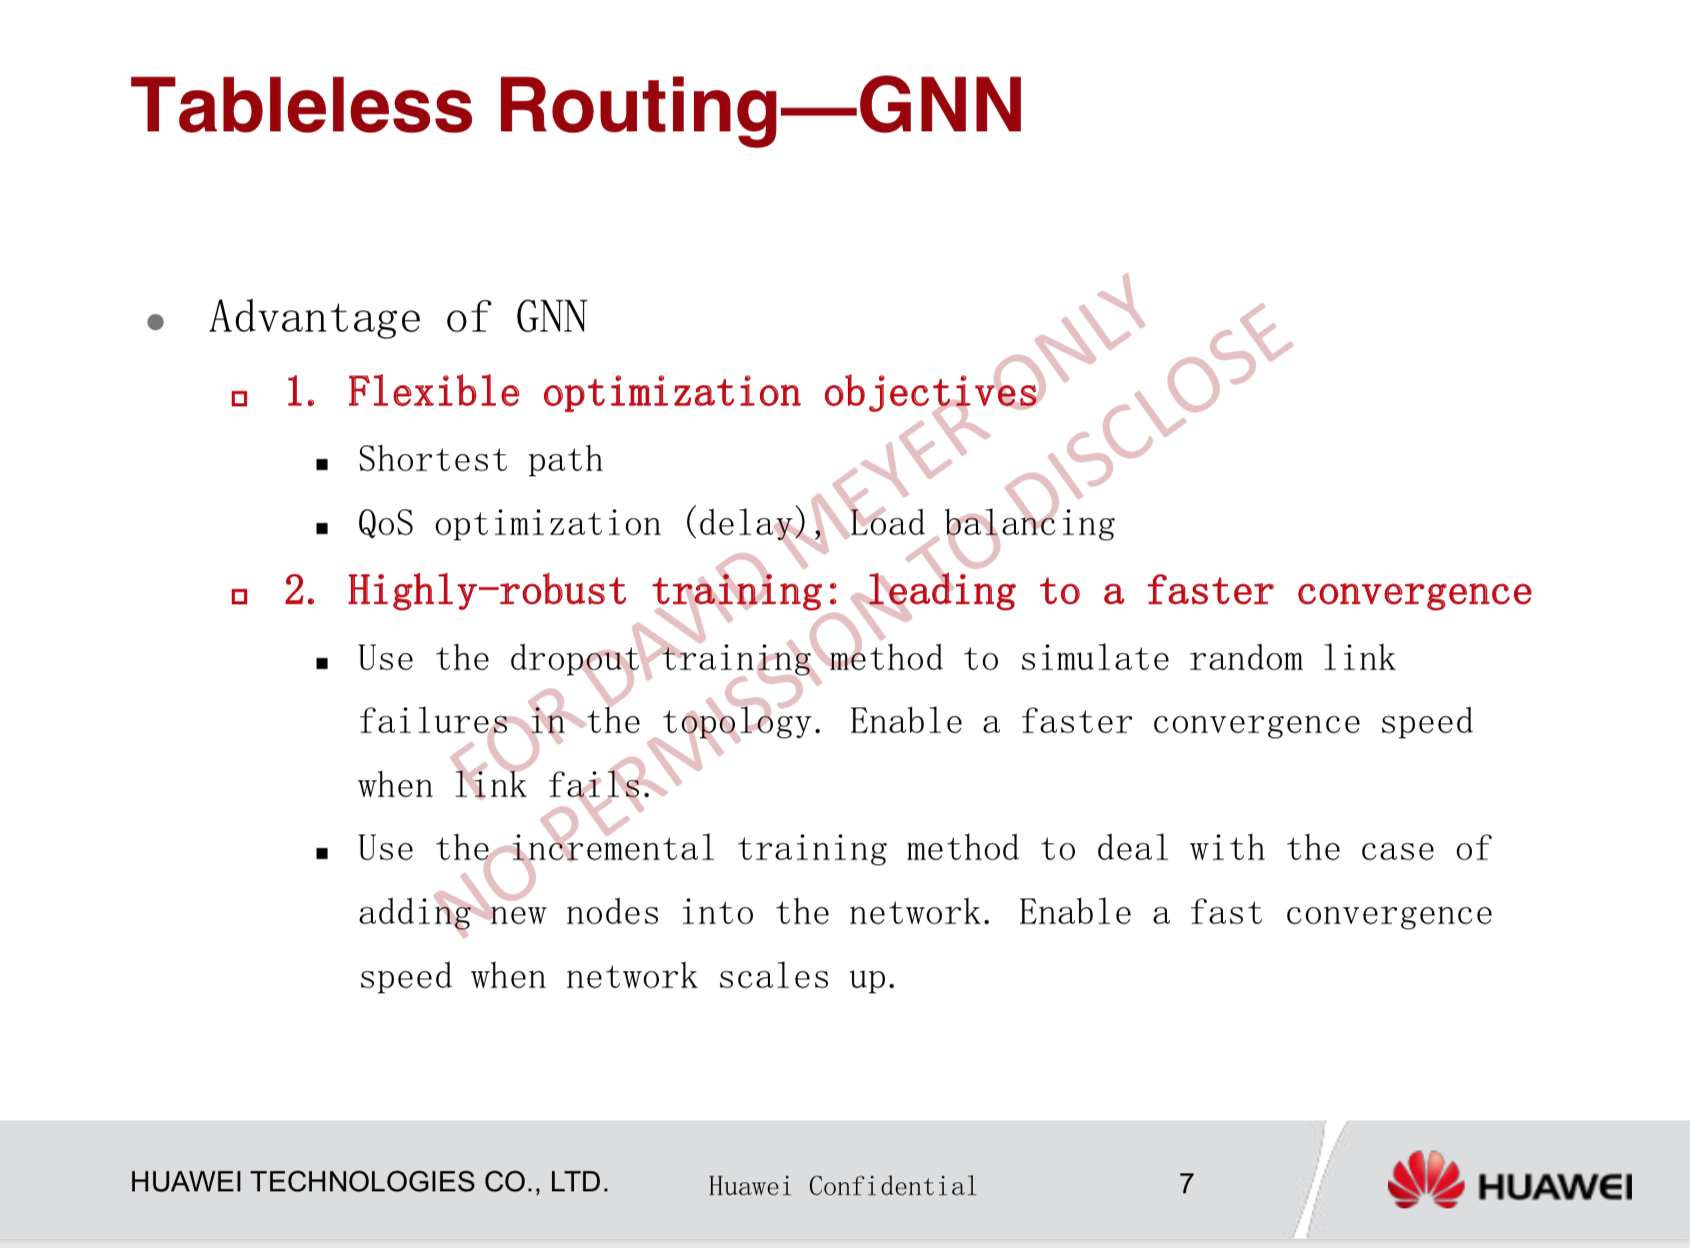
\includegraphics[scale=0.4, frame] {images/slide7.png}}
\caption{Slide 7}
\label{fig:slide7}
\end{figure}

\subsection{Possible Collaborators}
\label{slide6:possible_collaborators}
Both network hardware designers, machine learning people and network operators would be useful collaborators here. However, as I mentioned above 
(Section \ref{subsec:gnn} and \ref{subsec:table_size}), there are many issues that need to be resolved/supported.


\subsection{Marketing Strategies}
\label{slide6:marketing_strategies}
Again, in my opinion it is too early to start marketing activities.

\subsection{Nits}
\label{slide6:nits}
N/A

\begin{figure}[h]
\center{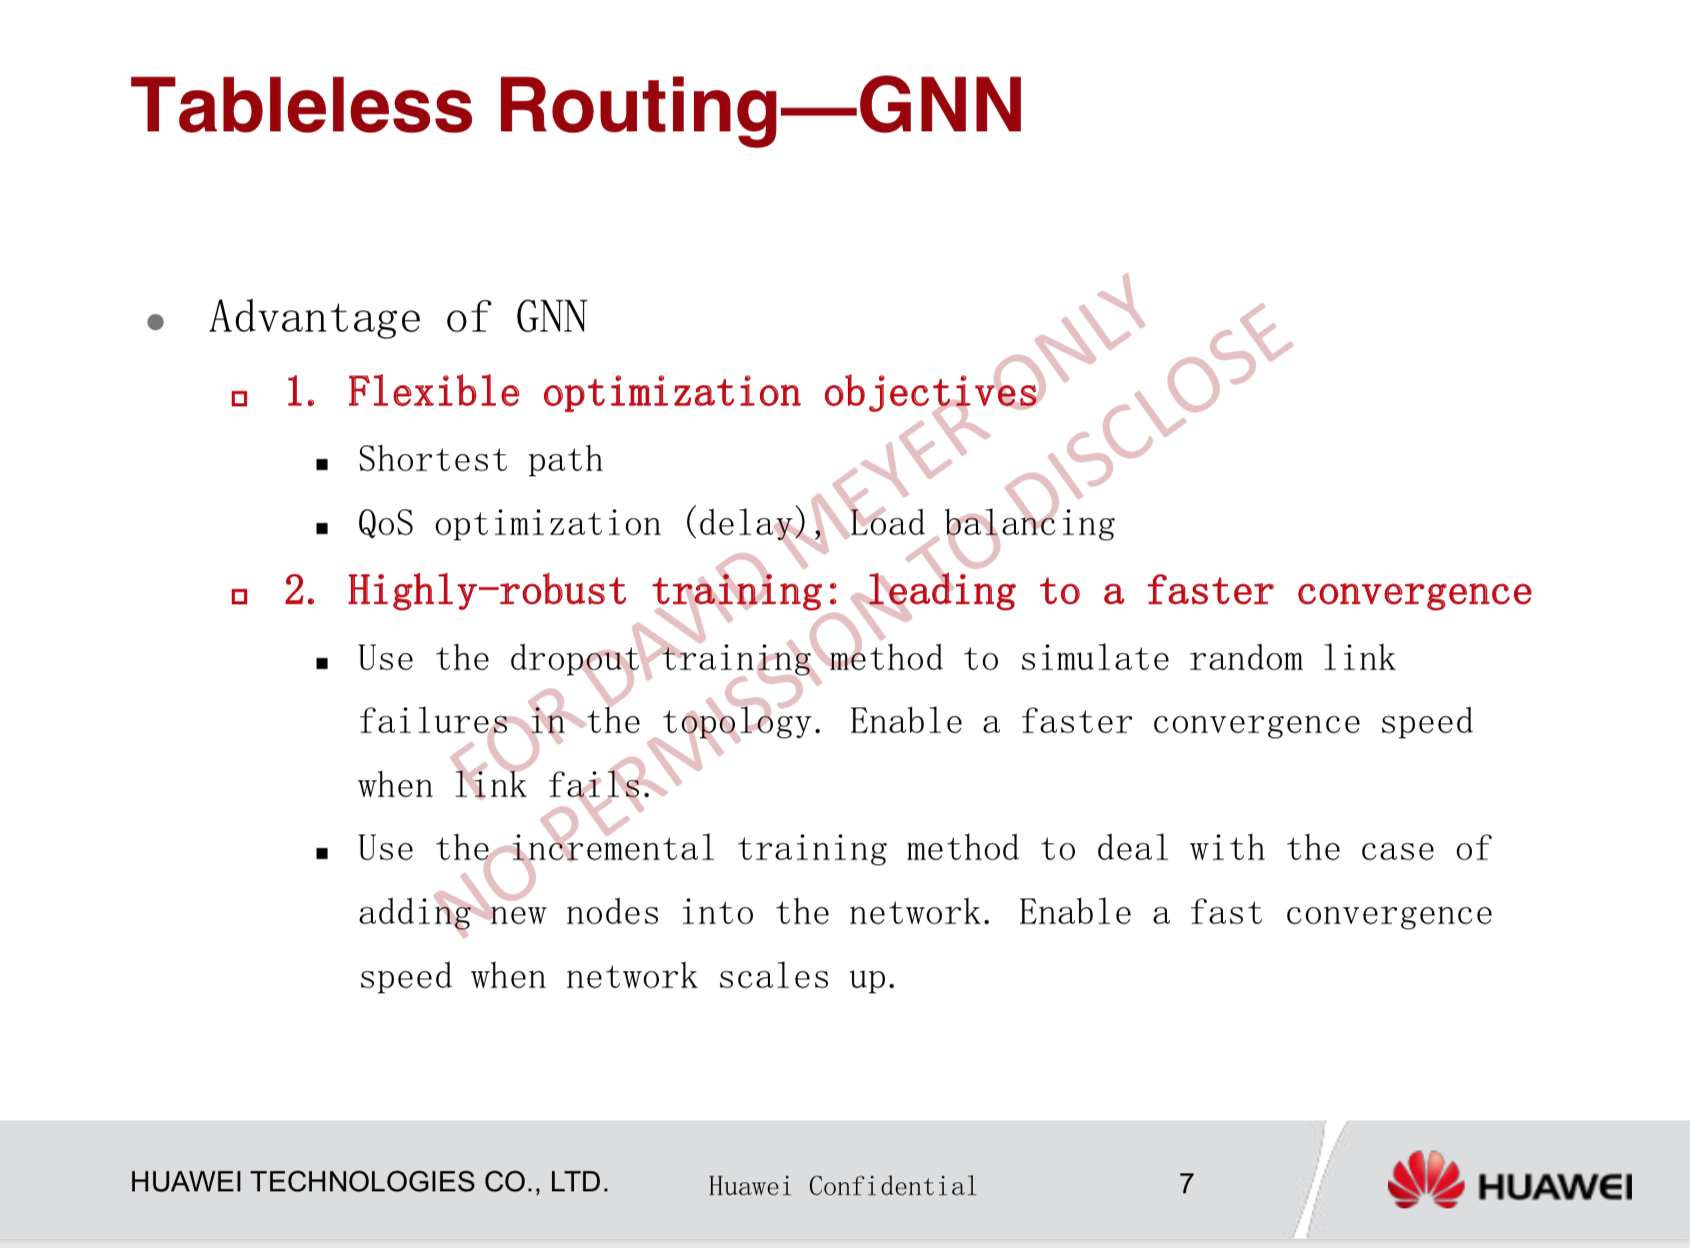
\includegraphics[scale=0.4, frame] {images/slide7.png}}
\caption{Slide 7}
\label{fig:slide7}
\end{figure}


\section{Slide 7}
\label{sec:slide7}
Slide 7 (Figure \ref{fig:slide7}) discusses the advantages of using a GNN to solve the routing problem.

\subsection{Technical Feedback}
\label{slide7:technical_feedback}
Bullet 1 on slide 7 discusses the flexibility of the method, mentioning that the method can do both 
shortest path (e.g., OSPF \cite{rfc2328}) and/or load balancing. Again, since you have to use OSPF (RIP \cite{rfc2453}, 
BGP \cite{rfc4271}, or others) to find the labels (output ports) to train the FFNN, a question one might ask is why all of the 
complexity of the GNN approach is really needed.


\begin{figure}
\center{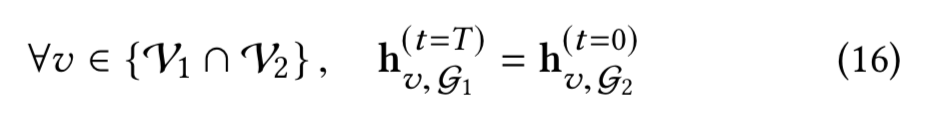
\includegraphics[scale=0.4, frame] {images/graph_update.png}}
\caption{Graph Update Procedue}
\label{fig:graph_update}
\end{figure}


\bigskip
\noindent
Bullet 2 discusses the use of dropout to simulate link and other failures, and the incremental training method for adding/subtracting 
nodes. There seems to be an error in \cite{DBLP:conf/sigcomm/GeyerC18} regarding incremental updates. In particular, Equation 16 
in \cite{DBLP:conf/sigcomm/GeyerC18}, shown in Figure \ref{fig:graph_update}, appears to be incorrect (it is backwards). That is,  it should say

\begin{equation}
\textbf{h}_{v, \mathcal{G}_2}^{(t = 0)} \coloneqq  \textbf{h}_{v, \mathcal{G}_1}^{(t = T)}
\label{eqn:h_update}
\end{equation}

\bigskip
\noindent
Note that I used $\coloneqq$ rather than $=$ in Equation \ref{eqn:h_update} because it is really an assignment of the initial state for the iterative process 
on $\mathcal{G}_2$.

\bigskip
\noindent
Finally, what isn't discussed here is the complexity of the update procedure, and where it would be executed.

\subsection{Possible Collaborators}
\label{slide7:possible_collaborators}
N/A

\subsection{Marketing Strategies}
\label{slide7:marketing_strategies}
N/A

\subsection{Nits}
\label{slide7:nits}
N/A


\section{Slide 8}
\label{sec:slide8}
Slide 8 reviews some of the key concepts of GNN routing and forwarding, focusing on "Neural network forwarding" (bullet 4). My first question
was about the details of the current (recent) plan, namely, using a "two-layer BNN (only XOR\&ADD required), supported by existing hardware 
(P4), with some precision loss". More detail on how and why this works would be useful.  Slide 9 shows how this might be implemented in P4.

\subsection{Technical Feedback}
\label{slide8:technical_feedback}
The most obvious question one might have here is whether the advantages of tableless routing (see Figure \ref{fig:slide7}) outweigh the additional
cost of on-board computational resources such as are proposed in the medium and longer term plans.


\subsection{Possible Collaborators}
\label{slide8:possible_collaborators}
As I've mentioned on other slides, the obvious collaborators would be service providers, machine learning academics, and other network engineers.

\subsection{Marketing Strategies}
\label{slide8:marketing_strategies}
N/A

\subsection{Nits}
\label{slide8:nits}
Slide 9 is a busy slide that tries to fill in some of the details. 



\section{Slide 10}
\label{sec:slide10}
Slide 10 introduces the reliability challenges with the GNN routing approach.


\subsection{Technical Feedback}
\label{slide10:technical_feedback}
The key issue here that while the approach has error rates of less that 5\% so that 95\% of node pairs learn the shortest path between them, the algorithm does
not provide guarantees for the remaining 5\% of pairs. This means, roughly, that each node has a probability $p < 0.05$ chance that a packet will be
misrouted \footnote{This misrouting can apparently result it routing loops, blackholes, and the like.}. As pointed out, the error rate is due to the probabilistic nature
of neural networks. 

\bigskip
\noindent
One of the innovations in this work is to borrow ideas from reachability assurance used in an IoT setting. In particular,  a \emph{Reliable Tableless Forwarding} (RTF)
method with a 100\% reachability guarantee is proposed.

\subsubsection{Aside: \emph{Route} vs.  \emph{Reachibility}}
\label{subsubsec:route_vs_reachability}
The slide states that RTF provides a 100\% reachability guarantee. Actually, routing doesn't provide reachability guarantees. For example, even if the route points to 
a correct interface at some time $t$,  existence of the route \emph{does not} guarantee reachability. That is, even if we know the correct next hop toward the destination,
any number of events can prevent a packet from getting to its destination; examples include ingress filtering, in which case choosing the wrong source address
\footnote{In the case of multi-homing.} can cause a packet which is sent on the correct interface towards the destination to be dropped, and many others.
 
 \bigskip
 \noindent
 Slide 11 overviews a Link Reversal Routing (LRR)  algorithm that converts a Directed Acyclic Graph (DAG) into a Destination-oriented DAG (DDAG). The interesting point here
 is that the algorithm can convert a DAG into a DDAG in a finite number of steps; however, the complexity of the algorithm isn't outlined. Slide 12 shows an implementation
 of the LRR algorithm.

\subsection{Possible Collaborators}
\label{slide10:possible_collaborators}
N/A

\subsection{Marketing Strategies}
\label{slide10:marketing_strategies}
N/A

\subsection{Nits}
\label{slide10:nits}
N/A

\section{Summary \& Conclusions}
\label{sec:conclusions}

The key features of Tableless Routing are summarized as follows (Slide 13):
\begin{itemize}
\item Minimized table storage requirements
\item  No computation-based forwarding
\item Flexible optimization objectives, e.g.
\begin{itemize}
\item Shortest-path routing
\item QoS routing of various forms
\end{itemize}
\item 100\% reachability guarantee for any number of link/node failures or neural network errors (if the network
is still connected after link/node failures)
\item Key technologies: GNN and Tableless LRR
\end{itemize}

\bigskip
\noindent
\subsubsection{Final Comments}
First, regarding routing table storage, lookup latency and algorithm complexity: as I mentioned in the introduction, is the overall routing table size problem compelling these days?
This is discussed in Section \ref{subsec:table_size}. Since the complexity of the solution appears to be significantly greater than say, computing shortest paths with 
Dijkstra's algorithm \cite{Ahuja:1990:FAS:77600.77615}, the significant additional complexity that Tableless LRR incurs needs stronger motivation.

\bigskip
\noindent
I also mentioned a few problems with the idea of using Graph Neural Networks for routing. First, the way nodes update their routing state is reminiscent of
distance-vector routing algorithms. As such one might expect classic distance-vector problems such as counting to infinity. Next, the authors use 
dropout \cite{Srivastava:2014:DSW:2627435.2670313}  to regularize the training of the GNN. The idea here is that dropping out random links during each 
training cycle, effectively models link failure. But does this approach effectively model link failure, and how would you show that this is true? Finally,  the generation
of the data labelled with output port (required to train the FFNN) requires the simulation of \emph{an existing routing protocol} on the graph (network)  So you need 
a routing protocol to find the output ports in the first place.

\bigskip
\noindent
There is an issue of \emph{route vs. reachability} as discussed in Section  \ref{subsubsec:route_vs_reachability}. The key point here is that the existence of 
a route to a destination (really the next-hop towards the destination) doesn't tell you that the destination is \emph{reachable}, so saying that there is a 
"100\% reachability guarantee" isn't really accurate.

\bigskip
\noindent
Another important observation here is that while the GNN formalism is an interesting approach to learning inference on a graph, it doesn't learn control \footnote{While one
might argue that the feedback in an RNN is a form of control, an RNN doesn't learn a \emph{policy} function $\pi: S \to A$.}.
For example, Equation 4 of  \cite{DBLP:conf/sigcomm/GeyerC18}:

\begin{flalign*}
\textbf{h}^{(t)}_v = f \bigg ( \Big \{ \textbf{h}^{(t - 1)}_{\text{Nbr}(v)} \Big \} \bigg) = \sum\limits_{u \in \text{Nbr}(v)} f^{*} \Big (\textbf{h}^{(t - 1)}_{u} \Big )
\end{flalign*}

\bigskip
\noindent
shows that the model doesn't really learn control; rather, the hidden state $\textbf{h}^{(t)}_v$ is hard-coded to be a function of $\text{Nbr}(v)$, the neighbors of node (router) $v$. 
In Reinforcement Learning (RL) parlance, the GNN model doe not learn a \emph{policy} $\pi$ such that  $\pi: S \to A$, where $S$ is the set of states and $A$ are the possible 
actions in state $S$. As such I would expect that the main competitors for routing approaches based on GNNs would be RL algorithms designed to learn optimized control. See, 
for example,  \cite{2017arXiv170803074V}.

\bigskip
\noindent
Finally, there is another problem with any data-driven approach that is particularly acute for routing problems: you don't see what happens to the data in the long term. 
More specifically, what looks good to your  metrics right now might kill the product in a few years. As a result, continual retraining \footnote{Such retraining will need to 
be incremental and capable of dealing with non-stationary distributions.}, perhaps along the lines of \cite{2018arXiv180310232I}, will be required. How exactly to do this 
and what data to use for this is still open problems.



\newpage
\bibliographystyle{ieeetr}
\bibliography{/Users/dmm/papers/huawei/bib/huawei.bib}



\end{document} 
